\section{Loading parameters}
The last important feature of the CPU library is to provide support for setting kernel parameters.
As seen in listing \ref{lst:kernel-constant}, this is implemented in the \verb/load_constant/ function.
The call takes an address and a value as parameters, as can be seen in listing \ref{lst:load-constant}

\begin{c-code}[caption=Setting a kernel parameter, label=lst:load-constant]
load_constant(0, 0x07E0);
\end{c-code}

\begin{figure}[H]
    \centering
    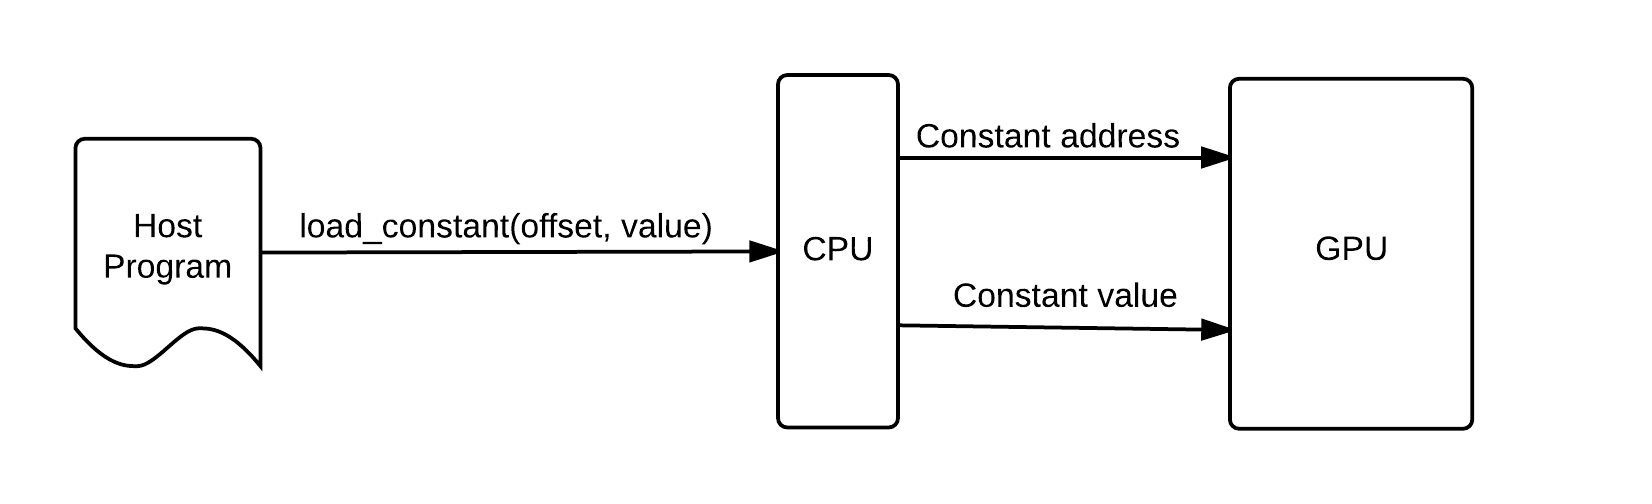
\includegraphics[width=\textwidth]{../cpu/diagrams/loading_a_constant.png}
    \caption{CPU-GPU interaction when loading a parameter.}
    \label{fig:loading_a_constant}
\end{figure}

The \verb/load_constant/ function is simply implemented by writing the constant value to the requested address.
